%%%%%%%%%%%%%%%%%%%%%%%%%%%%%%%%%%%%%%%%%%%%%%%%%%%%%%%%%%%%%%%%%%%%%%%%
%                                                                      %
%     File: Thesis_Results.tex                                         %
%     Tex Master: Thesis.tex                                           %
%                                                                      %
%     Author: Andre C. Marta                                           %
%     Last modified :  2 Jul 2015                                      %
%                                                                      %
%%%%%%%%%%%%%%%%%%%%%%%%%%%%%%%%%%%%%%%%%%%%%%%%%%%%%%%%%%%%%%%%%%%%%%%%

\chapter{Results}
\label{chapter:results}



\section{Constant Volatility Model}

\begin{figure}[h]
    \centering
    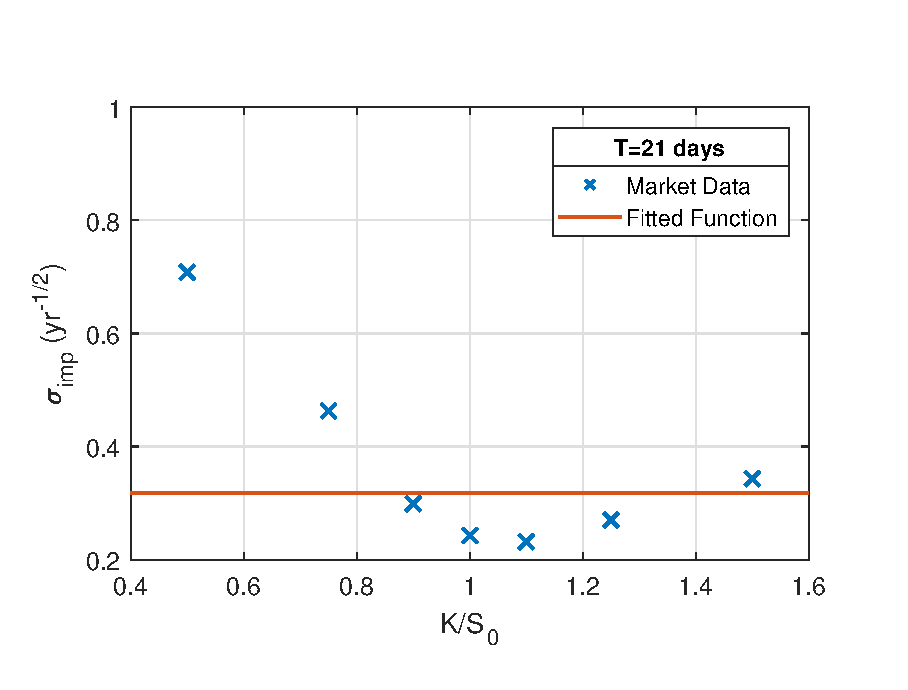
\includegraphics[width=.65\linewidth]{ConstVol1.eps}
    \caption[Implied volatility function fitted to the implied volatility data for maturity $T=21$ days under constant volatility model.]{Implied volatility function fitted to the implied volatility data for maturity $T=21$ days under constant volatility model.}\label{fig:CVT1}
\end{figure}   

\begin{table}[h]
    \centering
        \renewcommand{\arraystretch}{1.2}
\begin{tabular}{@{}lr@{}}
\toprule
 $\sigma_{imp,\mathrm{mdl}}$ ($\SI{}{\year\tothe{-1/2}}$) & Cost \\ \midrule
 0.3174 & 0.0635 \\
\bottomrule
\end{tabular}
  \caption[Fit results from constant volatility model for maturity $T=21$ days under constant volatility model.]{Fit results from constant volatility model for maturity $T=21$ days under constant volatility model.}
  \label{tab:CVRT1}
\end{table}


\begin{table}[h]
\centering
\renewcommand{\arraystretch}{1.2}
\begin{tabular}{@{}lcccccr@{}}
\toprule
$K$ ($\EUR$) & $\sigma_{imp,\mathrm{mkt}}$ ($\SI{}{\year\tothe{-1/2}}$) &  $\sigma_{imp,\mathrm{mdl}}$ ($\SI{}{\year\tothe{-1/2}}$) &$\Delta\sigma_{imp}/\sigma_{imp,\mathrm{mkt}}(\%)$&$C_{\mathrm{mkt}}$ ($\EUR$)&$C_{\mathrm{mdl}}$ ($\EUR$)& $\Delta C/C_{\mathrm{mkt}}(\%)$\\ \midrule
0.50 & 0.7082 & \multirow{7}{*}{0.3174} & 55.2 & 0.50001 & 0.50000 & 0.0026 \\
0.75 & 0.4632 &  & 31.5 & 0.25065 & 0.25002 & 0.3 \\
0.90 & 0.2989 &  & 6.2 & 0.10439 & 0.10540 & 1.0 \\
1.00 & 0.2425 &  & 30.9 & 0.02792 & 0.03654 & 30.9 \\
1.10 & 0.2314 &  & 37.1 & 2.42$\times10^{-3}$ & 7.41$\times10^{-3}$ & 205.9 \\
1.25 & 0.2699 &  & 17.6 & 5.34$\times10^{-5}$ & 25.01$\times10^{-5}$ & 367.9 \\
1.50 & 0.3433 &  & 7.5 & 5.75$\times10^{-7}$ & 1.12$\times10^{-7}$ & 80.5 \\ \bottomrule
\end{tabular}
  \caption[Comparison between fitted function and original data for maturity $T=21$ days under constant volatility model.]{Comparison between fitted function and original data for maturity $T=21$ days under constant volatility model.}
  \label{tab:CVT1}
\end{table}




\begin{figure}[h]
    \centering
    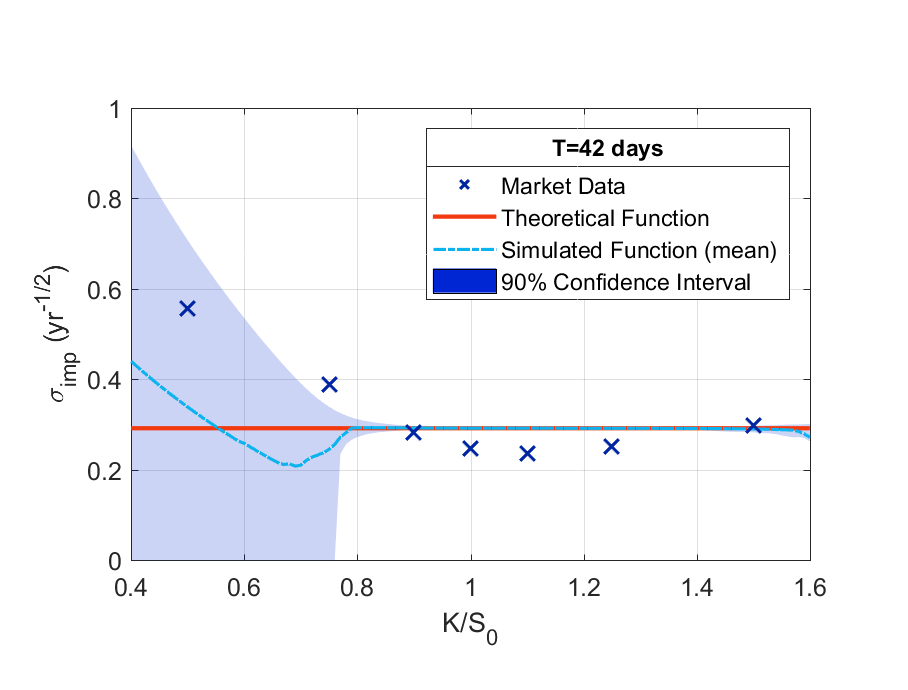
\includegraphics[width=.65\linewidth]{ConstVol2.eps}
    \caption[Implied volatility function fitted to the implied volatility data for maturity $T=42$ days under constant volatility model.]{Implied volatility function fitted to the implied volatility data for maturity $T=42$ days under constant volatility model.}\label{fig:CVT2}
\end{figure}   

\begin{table}[!htb]
    \centering
        \renewcommand{\arraystretch}{1.2}
\begin{tabular}{@{}lr@{}}
\toprule
 $\sigma_{imp,\mathrm{mdl}}$ ($\SI{}{\year\tothe{-1/2}}$) & Cost \\ \midrule
 0.2918 & 0.0282 \\
\bottomrule
\end{tabular}
  \caption[Fit results from constant volatility model for maturity $T=42$ days under constant volatility model.]{Fit results from constant volatility model for maturity $T=42$ days under constant volatility model.}
  \label{tab:CVRT2}
\end{table}

\begin{table}[h]
\centering
\renewcommand{\arraystretch}{1.2}
\begin{tabular}{@{}lcccccr@{}}
\toprule
$K$ ($\EUR$) & $\sigma_{imp,\mathrm{mkt}}$ ($\SI{}{\year\tothe{-1/2}}$) &  $\sigma_{imp,\mathrm{mdl}}$ ($\SI{}{\year\tothe{-1/2}}$) &$\Delta\sigma_{imp}/\sigma_{imp,\mathrm{mkt}}(\%)$&$C_{\mathrm{mkt}}$ ($\EUR$)&$C_{\mathrm{mdl}}$ ($\EUR$)& $\Delta C/C_{\mathrm{mkt}}(\%)$\\ \midrule
0.50 & 0.5556 & \multirow{7}{*}{0.2918} & 47.5 & 0.50005 & 0.50000 & 0.01 \\
0.75 & 0.3876 &  & 24.7 & 0.25186 & 0.25027 & 0.6 \\
0.90 & 0.2824 &  & 3.3 & 0.11069 & 0.11166 & 0.9 \\
1.00 & 0.2461 &  & 18.6 & 0.04006 & 0.04749 & 18.5 \\
1.10 & 0.2354 &  & 23.9 & 8.52$\times10^{-3}$ & 15.00$\times10^{-3}$ & 75.9 \\
1.25 & 0.2525 &  & 15.6 & 6.21$\times10^{-4}$ & 15.75$\times10^{-4}$ & 153.8 \\
1.50 & 0.2968 &  & 1.7 & 1.58$\times10^{-5}$ & 1.24$\times10^{-5}$ & 21.4 \\ \bottomrule
\end{tabular}
  \caption[Comparison between fitted function and original data for maturity $T=42$ days under constant volatility model.]{Comparison between fitted function and original data for maturity $T=42$ days under constant volatility model.}
  \label{tab:CVT2}
\end{table}




\begin{figure}[h]
    \centering
    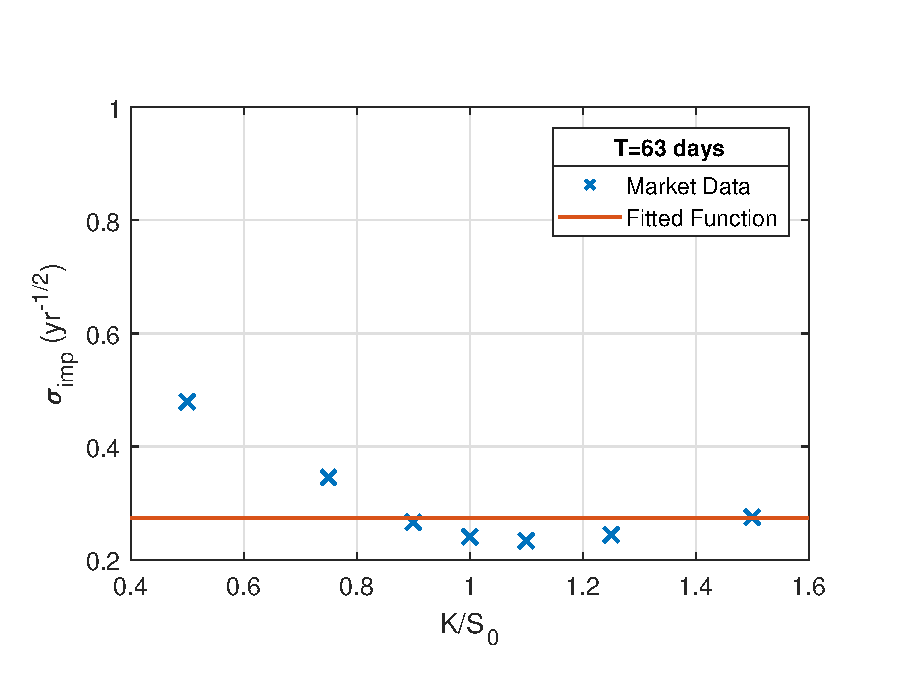
\includegraphics[width=.65\linewidth]{ConstVol3.eps}
    \caption[Implied volatility function fitted to the implied volatility data for maturity $T=63$ days under constant volatility model.]{Implied volatility function fitted to the implied volatility data for maturity $T=63$ days under constant volatility model.}\label{fig:CVT3}
\end{figure}   

\begin{table}[h]
    \centering
        \renewcommand{\arraystretch}{1.2}
\begin{tabular}{@{}lr@{}}
\toprule
 $\sigma_{imp,\mathrm{mdl}}$ ($\SI{}{\year\tothe{-1/2}}$) & Cost \\ \midrule
 0.2742 & 0.0164 \\
\bottomrule
\end{tabular}
  \caption[Fit results from constant volatility model for maturity $T=63$ days under constant volatility model.]{Fit results from constant volatility model for maturity $T=63$ days under constant volatility model.}
  \label{tab:CVRT3}
\end{table}

\begin{table}[h]
\centering
\renewcommand{\arraystretch}{1.2}
\begin{tabular}{@{}lcccccr@{}}
\toprule
$K$ ($\EUR$) & $\sigma_{imp,\mathrm{mkt}}$ ($\SI{}{\year\tothe{-1/2}}$) &  $\sigma_{imp,\mathrm{mdl}}$ ($\SI{}{\year\tothe{-1/2}}$) &$\Delta\sigma_{imp}/\sigma_{imp,\mathrm{mkt}}(\%)$&$C_{\mathrm{mkt}}$ ($\EUR$)&$C_{\mathrm{mdl}}$ ($\EUR$)& $\Delta C/C_{\mathrm{mkt}}(\%)$\\ \midrule
0.50 & 0.4789 &\multirow{7}{*}{0.2742}  & 42.7 & 0.50009 & 0.50000 & 0.02 \\
0.75 & 0.3452 &  & 20.6 & 0.25296 & 0.25077 & 0.9 \\
0.90 & 0.2658 &  & 3.2 & 0.11533 & 0.11650 & 1.0 \\
1.00 & 0.2401 &  & 14.2 & 0.04787 & 0.05465 & 14.2 \\
1.10 & 0.2330 &  & 17.7 & 0.01421 & 0.02069 & 45.5 \\
1.25 & 0.2438 &  & 12.5 & 1.80$\times10^{-3}$ & 3.33$\times10^{-3}$ & 85.1 \\
1.50 & 0.2749 &  & 0.3 & 7.66$\times10^{-5}$ & 7.44$\times10^{-5}$ & 2.9 \\ \bottomrule
\end{tabular}
  \caption[Comparison between fitted function and original data for maturity $T=63$ days under constant volatility model.]{Comparison between fitted function and original data for maturity $T=63$ days under constant volatility model.}
  \label{tab:CVT3}
\end{table}





\begin{figure}[h]
    \centering
    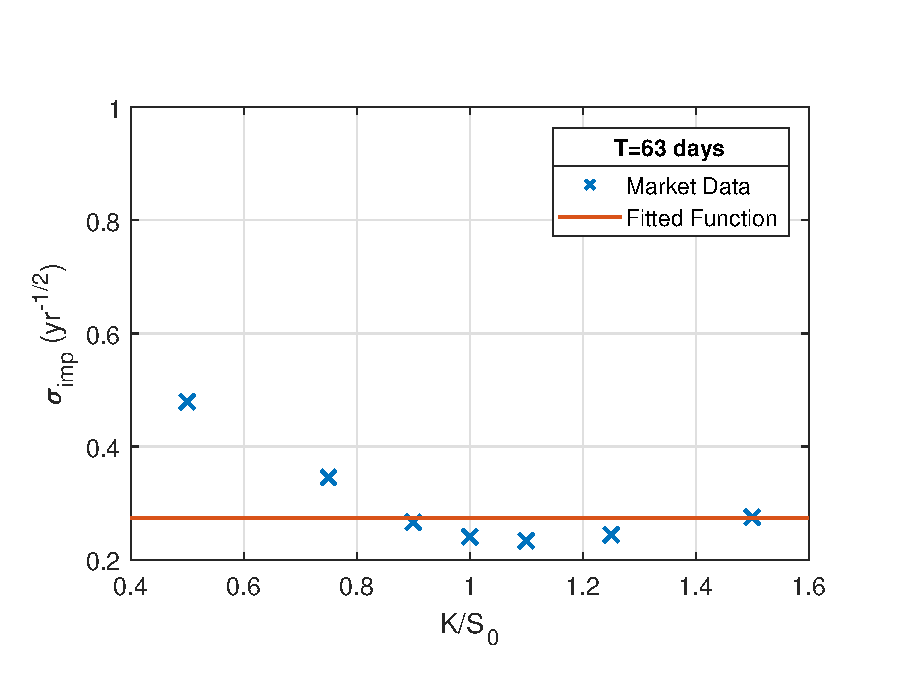
\includegraphics[width=.65\linewidth]{ConstVol3.eps}
    \caption[Implied volatility function fitted to the implied volatility data for maturity $T=126$ days under constant volatility model.]{Implied volatility function fitted to the implied volatility data for maturity $T=126$ days under constant volatility model.}\label{fig:CVT4}
\end{figure}   

\begin{table}[h]
    \centering
        \renewcommand{\arraystretch}{1.2}
\begin{tabular}{@{}lr@{}}
\toprule
 $\sigma_{imp,\mathrm{mdl}}$ ($\SI{}{\year\tothe{-1/2}}$) & Cost \\ \midrule
0.2518 & 0.0069 \\
\bottomrule
\end{tabular}
  \caption[Fit results from constant volatility model for maturity $T=126$ days under constant volatility model.]{Fit results from constant volatility model for maturity $T=126$ days under constant volatility model.}
  \label{tab:CVRT4}
\end{table}


\begin{table}[h]
\centering
\renewcommand{\arraystretch}{1.2}
\begin{tabular}{@{}lcccccr@{}}
\toprule
$K$ ($\EUR$) & $\sigma_{imp,\mathrm{mkt}}$ ($\SI{}{\year\tothe{-1/2}}$) &  $\sigma_{imp,\mathrm{mdl}}$ ($\SI{}{\year\tothe{-1/2}}$) &$\Delta\sigma_{imp}/\sigma_{imp,\mathrm{mkt}}(\%)$&$C_{\mathrm{mkt}}$ ($\EUR$)&$C_{\mathrm{mdl}}$ ($\EUR$)& $\Delta C/C_{\mathrm{mkt}}(\%)$\\ \midrule
0.50 & 0.3878 &  \multirow{7}{*}{0.2518}& 35.1 & 0.50035 & 0.50000 & 0.07 \\
0.75 & 0.2954 &  & 14.7 & 0.25694 & 0.25344 & 1.4 \\
0.90 & 0.2444 &  & 3.1 & 0.12716 & 0.12882 & 1.3 \\
1.00 & 0.2295 &  & 9.7 & 0.06467 & 0.07094 & 9.7 \\
1.10 & 0.2269 &  & 11.0 & 0.02862 & 0.03488 & 21.9 \\
1.25 & 0.2340 &  & 7.6 & 7.57$\times10^{-3}$ & 9.98$\times10^{-3}$ & 31.8 \\
1.50 & 0.2521 &  & 0.1 & 8.58$\times10^{-4}$ & 8.51$\times10^{-4}$ & 0.8 \\ \bottomrule 
\end{tabular}
  \caption[Comparison between fitted function and original data for maturity $T=126$ days under constant volatility model.]{Comparison between fitted function and original data for maturity $T=126$ days under constant volatility model.}
  \label{tab:CVT4}
\end{table}









\section{Static SABR Model}
\begin{figure}[h]
    \centering
    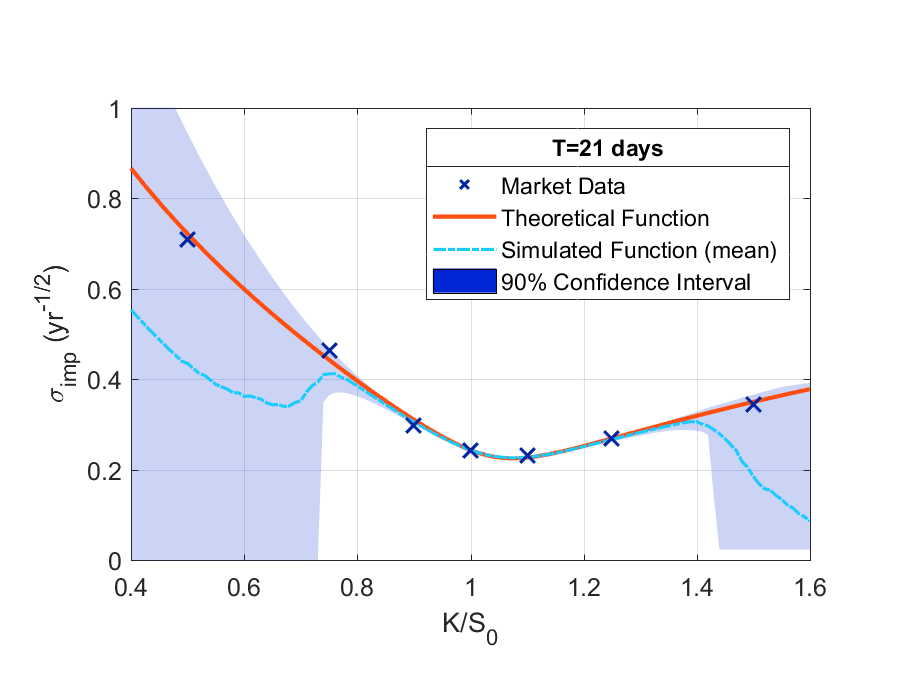
\includegraphics[width=0.65\linewidth]{SSABR1.eps}
    \caption[Implied volatility function fitted to the implied volatility data for maturity $T=21$ days under static SABR model.]{Implied volatility function fitted to the implied volatility data for maturity $T=21$ days under static SABR model.}\label{fig:SST1}
\end{figure}  


\begin{table}[h]
    \centering
        \renewcommand{\arraystretch}{1.2}
\begin{tabular}{@{}lcccr@{}}
\toprule
 $\alpha$ ($\SI{}{\year\tothe{-1/2}}$) & $\beta$ & $\rho$ & $\nu$ & Cost \\ \midrule
0.2381 &   0.3766 & -0.3760 & 2.1022 &  0.000415 \\
\bottomrule
\end{tabular}
  \caption[Fit results from constant volatility model for maturity $T=21$ days under static SABR model.]{Fit results from constant volatility model for maturity $T=21$ days under static SABR model.}
  \label{tab:SSRT1}
\end{table}  


\begin{table}[h]
\centering
\renewcommand{\arraystretch}{1.2}
\begin{tabular}{@{}lcccccr@{}}
\toprule
$K$ ($\EUR$) & $\sigma_{imp,\mathrm{mkt}}$ ($\SI{}{\year\tothe{-1/2}}$) &  $\sigma_{imp,\mathrm{mdl}}$ ($\SI{}{\year\tothe{-1/2}}$) &$\Delta\sigma_{imp}/\sigma_{imp,\mathrm{mkt}}(\%)$&$C_{\mathrm{mkt}}$ ($\EUR$)&$C_{\mathrm{mdl}}$ ($\EUR$)& $\Delta C/C_{\mathrm{mkt}}(\%)$\\ \midrule
0.50 & 0.7082 & 0.7209 & 1.8 & 0.50001 & 0.50002 & 0.001 \\
0.75 & 0.4632 & 0.4428 & 4.4 & 0.25065 & 0.25047 & 0.1 \\
0.90 & 0.2989 & 0.3105 & 3.9 & 0.10439 & 0.10501 & 0.6 \\
1.00 & 0.2425 & 0.2435 & 0.4 & 0.02792 & 0.02804 & 0.4 \\
1.10 & 0.2314 & 0.2269 & 2.0 & 2.42$\times10^{-3}$ & 2.23$\times10^{-3}$ & 8.0 \\
1.25 & 0.2699 & 0.2692 & 0.3 & 5.34$\times10^{-5}$ & 5.18$\times10^{-5}$ & 3.0 \\
1.50 & 0.3433 & 0.3500 & 1.9 & 5.75$\times10^{-7}$ & 8.32$\times10^{-7}$ & 44.7 \\ \bottomrule
\end{tabular}
  \caption[Comparison between fitted function and original data for maturity $T=21$ days under static SABR model.]{Comparison between fitted function and original data for maturity $T=21$ days under static SABR model.}
  \label{tab:SST1}
\end{table}






\begin{figure}[h]
    \centering
    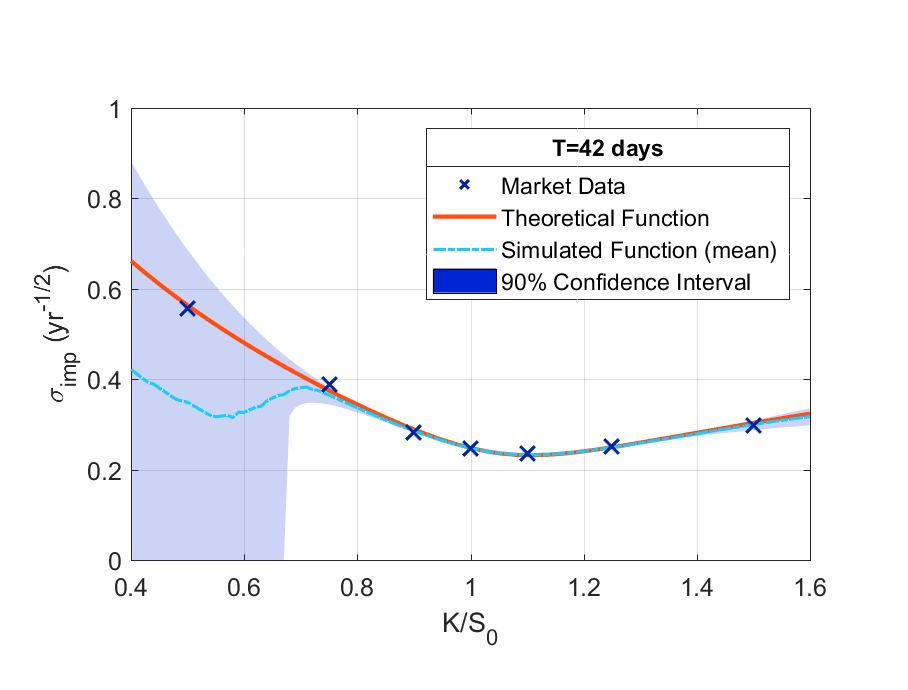
\includegraphics[width=0.65\linewidth]{SSABR2.eps}
    \caption[Implied volatility function fitted to the implied volatility data for maturity $T=42$ days under static SABR model.]{Implied volatility function fitted to the implied volatility data for maturity $T=42$ days under static SABR model.}\label{fig:SST2}
\end{figure}  


\begin{table}[h]
    \centering
        \renewcommand{\arraystretch}{1.2}
\begin{tabular}{@{}lcccr@{}}
\toprule
 $\alpha$ ($\SI{}{\year\tothe{-1/2}}$) & $\beta$ & $\rho$ & $\nu$ & Cost \\ \midrule
0.2434 & 0.7362 & -0.3664 & 1.4451& 0.000166\\
\bottomrule
\end{tabular}
  \caption[Fit results from constant volatility model for maturity $T=42$ days under static SABR model.]{Fit results from constant volatility model for maturity $T=42$ days under static SABR model.}
  \label{tab:SSRT2}
\end{table}  


\begin{table}[h]
\centering
\renewcommand{\arraystretch}{1.2}
\begin{tabular}{@{}lcccccr@{}}
\toprule
$K$ ($\EUR$) & $\sigma_{imp,\mathrm{mkt}}$ ($\SI{}{\year\tothe{-1/2}}$) &  $\sigma_{imp,\mathrm{mdl}}$ ($\SI{}{\year\tothe{-1/2}}$) &$\Delta\sigma_{imp}/\sigma_{imp,\mathrm{mkt}}(\%)$&$C_{\mathrm{mkt}}$ ($\EUR$)&$C_{\mathrm{mdl}}$ ($\EUR$)& $\Delta C/C_{\mathrm{mkt}}(\%)$\\ \midrule
0.50 & 0.5556 & 0.5631 & 1.4 & 0.50005 & 0.50006 & 0.002 \\
0.75 & 0.3876 & 0.3751 & 3.2 & 0.25186 & 0.25155 & 0.1 \\
0.90 & 0.2824 & 0.2891 & 2.4 & 0.11069 & 0.11139 & 0.6 \\
1.00 & 0.2461 & 0.2481 & 0.8 & 0.04006 & 0.04039 & 0.8 \\
1.10 & 0.2354 & 0.2322 & 1.4 & 8.52$\times10^{-3}$ & 8.19$\times10^{-3}$ & 3.9 \\
1.25 & 0.2525 & 0.2497 & 1.1 & 6.21$\times10^{-4}$ & 5.75$\times10^{-4}$ & 7.4 \\
1.50 & 0.2968 & 0.3033 & 2.2 & 1.58$\times10^{-5}$ & 2.12$\times10^{-5}$ & 33.9 \\ \bottomrule
\end{tabular}
  \caption[Comparison between fitted function and original data for maturity $T=42$ days under static SABR model.]{Comparison between fitted function and original data for maturity $T=42$ days under static SABR model.}
  \label{tab:SST2}
\end{table}






\begin{figure}[h]
    \centering
    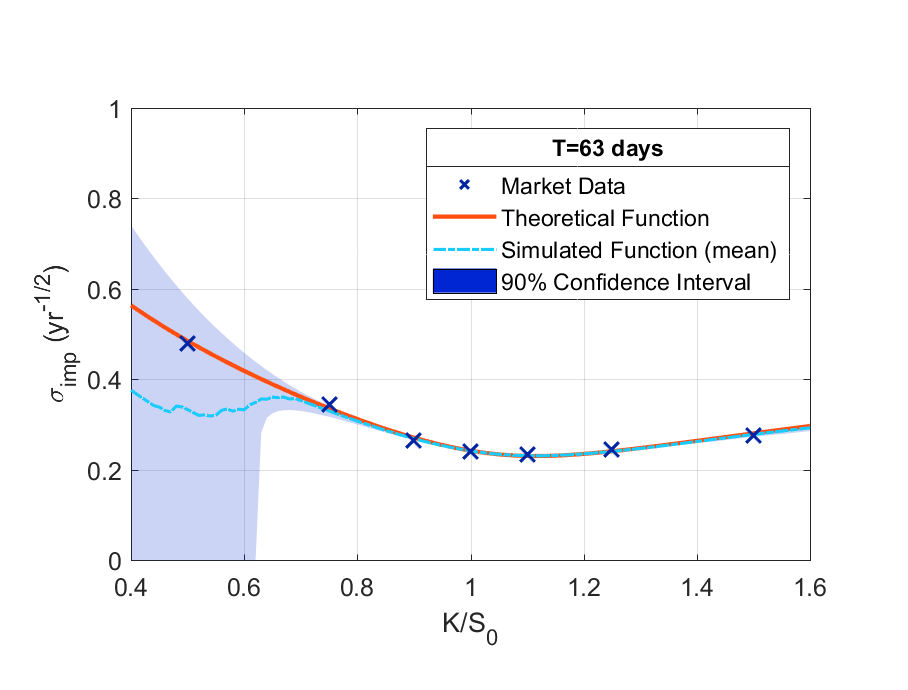
\includegraphics[width=0.65\linewidth]{SSABR3.eps}
    \caption[Implied volatility function fitted to the implied volatility data for maturity $T=63$ days under static SABR model.]{Implied volatility function fitted to the implied volatility data for maturity $T=63$ days under static SABR model.}\label{fig:SST3}
\end{figure}  


\begin{table}[h]
    \centering
        \renewcommand{\arraystretch}{1.2}
\begin{tabular}{@{}lcccr@{}}
\toprule
 $\alpha$ ($\SI{}{\year\tothe{-1/2}}$) & $\beta$ & $\rho$ & $\nu$ & Cost \\ \midrule
0.2375 & 0.7750 & -0.3119 & 1.1420 & 0.000102\\
\bottomrule
\end{tabular}
  \caption[Fit results from constant volatility model for maturity $T=63$ days under static SABR model.]{Fit results from constant volatility model for maturity $T=63$ days under static SABR model.}
  \label{tab:SSRT3}
\end{table}  


\begin{table}[h]
\centering
\renewcommand{\arraystretch}{1.2}
\begin{tabular}{@{}lcccccr@{}}
\toprule
$K$ ($\EUR$) & $\sigma_{imp,\mathrm{mkt}}$ ($\SI{}{\year\tothe{-1/2}}$) &  $\sigma_{imp,\mathrm{mdl}}$ ($\SI{}{\year\tothe{-1/2}}$) &$\Delta\sigma_{imp}/\sigma_{imp,\mathrm{mkt}}(\%)$&$C_{\mathrm{mkt}}$ ($\EUR$)&$C_{\mathrm{mdl}}$ ($\EUR$)& $\Delta C/C_{\mathrm{mkt}}(\%)$\\ \midrule
0.50 & 0.4789 & 0.4845 & 1.2 & 0.50009 & 0.50011 & 0.002 \\
0.75 & 0.3452 & 0.3357 & 2.8 & 0.25296 & 0.25256 & 0.2 \\
0.90 & 0.2658 & 0.2710 & 2.0 & 0.11533 & 0.11605 & 0.6 \\
1.00 & 0.2401 & 0.2421 & 0.8 & 0.04787 & 0.04826 & 0.8 \\
1.10 & 0.2330 & 0.2305 & 1.1 & 0.01421 & 0.01384 & 2.6 \\
1.25 & 0.2438 & 0.2409 & 1.2 & 1.80$\times10^{-3}$ & 1.68$\times10^{-3}$ & 6.7 \\
1.50 & 0.2749 & 0.2804 & 2.0 & 7.66$\times10^{-5}$ & 9.56$\times10^{-5}$ & 24.8 \\ \bottomrule
\end{tabular}
  \caption[Comparison between fitted function and original data for maturity $T=63$ days under static SABR model.]{Comparison between fitted function and original data for maturity $T=63$ days under static SABR model.}
  \label{tab:SST3}
\end{table}





\begin{figure}[h]
    \centering
    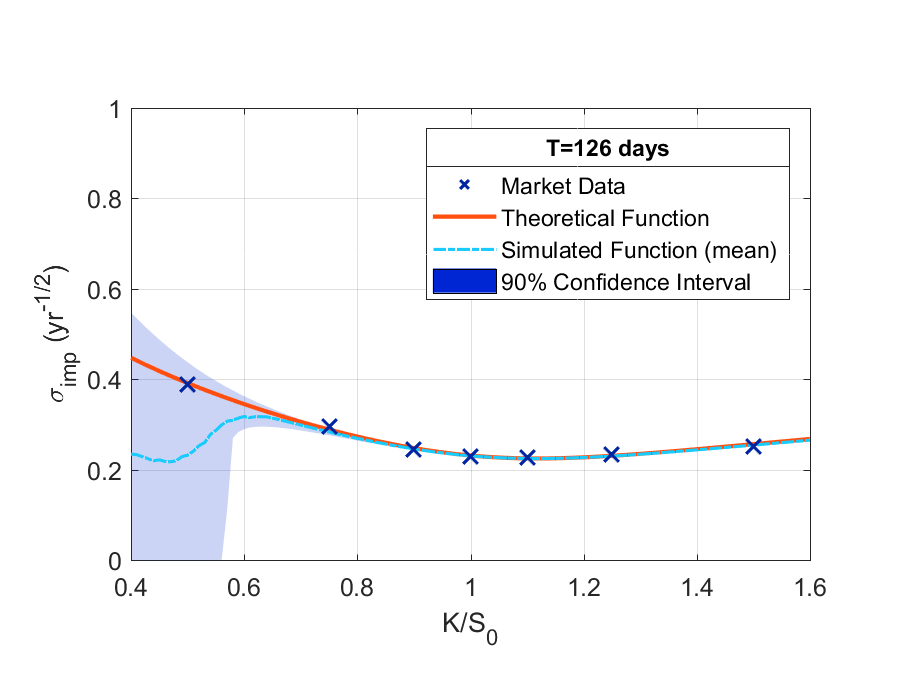
\includegraphics[width=0.65\linewidth]{SSABR4.eps}
    \caption[Implied volatility function fitted to the implied volatility data for maturity $T=126$ days under static SABR model.]{Implied volatility function fitted to the implied volatility data for maturity $T=126$ days under static SABR model.}\label{fig:SST4}
\end{figure}  


\begin{table}[h]
    \centering
        \renewcommand{\arraystretch}{1.2}
\begin{tabular}{@{}lcccr@{}}
\toprule
 $\alpha$ ($\SI{}{\year\tothe{-1/2}}$) & $\beta$ & $\rho$ & $\nu$ & Cost \\ \midrule
0.2267 & 0.8771 & -0.2383 & 0.8215 & 0.000055\\
\bottomrule
\end{tabular}
  \caption[Fit results from constant volatility model for maturity $T=126$ days under static SABR model.]{Fit results from constant volatility model for maturity $T=126$ days under static SABR model.}
  \label{tab:SSRT4}
\end{table}  


\begin{table}[h]
\centering
\renewcommand{\arraystretch}{1.2}
\begin{tabular}{@{}lcccccr@{}}
\toprule
$K$ ($\EUR$) & $\sigma_{imp,\mathrm{mkt}}$ ($\SI{}{\year\tothe{-1/2}}$) &  $\sigma_{imp,\mathrm{mdl}}$ ($\SI{}{\year\tothe{-1/2}}$) &$\Delta\sigma_{imp}/\sigma_{imp,\mathrm{mkt}}(\%)$&$C_{\mathrm{mkt}}$ ($\EUR$)&$C_{\mathrm{mdl}}$ ($\EUR$)& $\Delta C/C_{\mathrm{mkt}}(\%)$\\ \midrule
0.50 & 0.3878 & 0.3914 & 0.9 & 0.50035 & 0.50038 & 0.006 \\
0.75 & 0.2954 & 0.2887 & 2.2 & 0.25694 & 0.25633 & 0.2 \\
0.90 & 0.2444 & 0.2479 & 1.5 & 0.12716 & 0.12794 & 0.6 \\
1.00 & 0.2295 & 0.2314 & 0.8 & 0.06467 & 0.06522 & 0.8 \\
1.10 & 0.2269 & 0.2251 & 0.8 & 0.02862 & 0.02817 & 1.6 \\
1.25 & 0.2340 & 0.2309 & 1.3 & 7.57$\times10^{-3}$ & 7.18$\times10^{-3}$ & 5.2 \\
1.50 & 0.2521 & 0.2567 & 1.8 & 8.58$\times10^{-4}$ & 9.82$\times10^{-4}$ & 14.5 \\ \bottomrule
\end{tabular}
  \caption[Comparison between fitted function and original data for maturity $T=126$ days under static SABR model.]{Comparison between fitted function and original data for maturity $T=126$ days under static SABR model.}
  \label{tab:SST4}
\end{table}




\hl{show data and mention where it came from. confidentiality, etc}

\hl{in annex, should plot y-axes with different limits?}

\hl{should we include the market values in all comparison tables?}

\hl{plot surface function}

\hl{put units in fitted parameters}

\hl{crop images}